\documentclass{article}

\usepackage{setup}

\newsource{\sBook}{}{Taigen Daniel Leighton and Shohaku Okumura, translators.
  \emph{D\=ogen's Pure Standards for the Zen Community: A Translation of
    \emph{Eihei Shingi}}. State University of New York Press, 1996.}

\begin{document}

\chapter{Zen Meals under Dōgen's Pure Standards}

\raggedcolumns
\begin{multicols}{2}

\section{Introduction to \emph{Eihei Shingi}}

\emph{Eihei Shingi}, Eihei's Pure Standards, is a collection of essays
written by Eihei D\=ogen (1200--1253), the founder of the Soto branch
of Japanese Zen Buddhism. Unlike some of his other writings, more
focused on philosophy and the nature of reality, \emph{Eihei Shingi}
is primarily a book about day-to-day monastic practice, specifying
many rules, guidelines, and procedures. At the same time, this
ritualized way of life is presented not as arbitrary minutiae but as an
important part of religious practice, and many of these same practices
are still carried out by monks in Japan and elsewhere today.

The essay this class is based on, ``The Dharma for Taking Food'', was
written in 1246. It's concerned with the proper procedure for
breakfast and lunch meals at the monastery. (Dinner is not considered
a formal meal, but informal ``medicine'' to keep the body functioning
well.) It precisely specifies everything from the way to enter the
hall to the way of laying out your bowls as a series of precise
steps. This ritualized practice might seem extremely rigid to a
secular modern reader, but mealtime is a part of a monk's practice
just like sitting or walking meditation. D\=ogen says ``[F]ood is
the dharma of all dharmas, which only a buddha together with a buddha
can exhaustively penetrate. Just at such a time, there are the genuine
marks, nature, substance, power, function, causes. and conditions. For
this reason, dharma is itself food, food is itself dharma. This dharma
is what is received and used by all buddhas in the past and
future. This food is the fulfillment that is the joy of dharma and the
delight of meditation.'' Clearly, meals are a significant part of a
monk's path towards enlightenment.

At the same time, the specific prohibitions D\=ogen gives can be
amusing for a modern reader. Admonitions to not let dandruff fall in
your food or hide your food to get more suggest the image that monks
would otherwise do so left to their own devices.

While it may not free you from the illusions of the world, I hope
in this class to give you some sense about what life in a Kamakura Period
Zen monastery might have been like.

\section{Materials}

\begin{itemize}
\item Four or five nesting bowls
\item Bowl stand for largest bowl
\item Wrapping cloth
\item Bowl-wiping cloth (1.2 shaku (feet) long, a standard loom width)
\item Lap cloth
\item Place mat
\item Utensil bag
\item Spoon
\item Chopsticks
\item Cleaning stick
\end{itemize}

\section{Procedure}

\subsection{Entering}

\begin{itemize}
\item Signal sounds: night's end signal for breakfast, or three drum beats
and a large bell for lunch.
\item Monks wash hands and approach hall formally.
\item Three roll-downs are sounded on the hanging wooden block.
\item Monks enter hall silently in gassh\=o, starting with the left foot.
  When entering through the main entrance,
  ordinary monks enter the left side; the abbot enters
  through the right side (or through the center starting with the right
  foot).\footnote{Monks entering through the back enter on the left or right
    and with their left or right foot based on where they're sitting.}
\item Bow to Manjushri.
\item Approach your seat.
\item Bow to your seat, understood as a bow to those on each side, then
  turn clockwise and bow to the seat across from yours.
\item Tuck your left sleeve under your arm with your right hand, and vice versa.
\item Lift your the front of your okesa with both hands and hold it up in
  your left hand.
\item Sit on the platform, leaving your
  slippers behind, while steadying yourself with your right hand.
  Sit with your left leg on your right thigh.\footnote{in the half-lotus
    position}
\item Spread the okesa to cover your knees without your robe showing,
  keeping a bowl's width between yourself and the j\=oen, the
  edge of the platform for bowls.
\item The wooden fish is hit. After this point, latecomers are not allowed.
\end{itemize}

\subsection{Setting Out Bowls}

\begin{itemize}
\item The cloud-shaped gong in front of the kitchen is hit. Monks stand up, turn
clockwise to face the back of the seat. Gassh\=o with your head in a slight
bow. Hold your bowls in your left hand and unhook them with your right, then
carry them with both hands at chest height. Turn, bend down and sit, placing
your bowls behind your seat to the left, being mindful of your neighbors.
\item A monk makes a meal offering to Manjushri, proceeding in gassh\=o
  in front of another monk carrying a tray of food. The monk presents the
  food, bows at the front of the bowing mat, uncovers the eight-sided block,
  returns to the bowing mat and bows.
\item Three roll-downs on a drum; when the third is almost finished, the small
  bell in front of the hall is rung.
\item The abbot enters, and the monks get down from their platforms.
  The abbot bows to Manjushri and the assembly, then sits; the monks
  then bow in the same way. The abbot's attendants bow; one brings a
  table, bows, and leaves. The abbot's bowls are placed on this table.
\item Monks get back on the platform, leaving their slippers, and sit
  upright on zafus.
\item Monks hold up bowls at face height then place them down in front of
  them.
\item The supervisor enters, bows, offers incense to Manjushri, bows,
  goes in gassh\=o to the eight-sided block, bows, optionally hits it once.
\item Gassh\=o.
\item Untie the knot on the wrapping cloth.
\item Fold the bowl-wiping cloth, once horizontally and into three layers
  vertically.
\item Place the wiping cloth horizontally between yourself and the bowls
  and place the utensil bag above it.
\item Place the lap cloth over your knees.
\item Open the wrapping cloth, with the back corner out over the edge
of the platform and the front corner folded partly under itself. Then
the side corners should be folded under as far in as the bowl.
\item With both hands, open the place mat. Hold the place mat in your
  right hand, lift the bowls with your left hand, set down the place mat
  on the wrapping cloth, and then set the bowls on it.
\item Remove each bowl with both thumbs and set them out silently, starting
  with the smallest. (If your seat is a little too narrow, only put out
  three bowls.)
\item Open the utensil bag and remove the chopsticks, then the spoon, placing
them behind the bowls, points left.
\item Take the cleaning stick and place it between the second and third
  bowls, handle away from you.
\item Fold up the utensil bag and put it with the wiping cloth behind
  the bowls, under or behind the place mat.
\end{itemize}

\subsection{Opening Recitations}

\begin{itemize}
\item The supervisor hits the eight-sided block and says ``Humbly
  we consider the three treasures, may they acknowledge us.''
\item Monks gassh\=o and chant the Ten Names of Buddha (see texts).
\item The eight-sided block is struck.
\item The head monk chants the meal offering verse in gassh\=o, extending
each tone.
\item The junior monk who announces the meal enters and bows to Manjushri,
the abbot, and then the head monk. He stands at the end of the platform by
the left side of the entrance in shashu and announces the meal clearly.
\end{itemize}

\subsection{Serving}

\begin{itemize}
\item Servers offer food starting with the head monk and proceeding in
  order, ending with the abbot.
\item Servers bow humbly.
\item When serving soup or gruel, shake the ladle a few times and pause
  to avoid spilling, bending over and with your other hand against your chest.
\item Servers should give each monk the amount of food they want.
\item Monks should accept food respectfully, lifting their bowl with
  both hands and holding it low and level.
\item Signal with your hand when you have enough food, not taking more than
  you will eat.
\item When everyone has been served, the supervisor will hit the eight-sided
  block.
\item Gassh\=o and bow to the food, then do the five contemplations.
\item At lunch, take seven grains of rice with the thumb and first
  finger of your right hand and put them on the handle of your
  cleaning stick or the edge of your place mat as spirit
  offerings.\footnote{If rice is not served, offer at most the size of
    half a large coin.}
\item Gassh\=o and remain still.
\end{itemize}

\subsection{Eating}

\begin{itemize}
\item Eat with your spoon pointed straight into your mouth.\footnote{We
were told at the monastery that the spoon handle points directly towards
Buddha.}
\item Fully appreciate and contemplate the dharma of the principle of the Way
not to waste a single grain.
\end{itemize}

\subsubsection{Breakfast}
\begin{itemize}
\item Take your second bowl with your right hand and place it flat on
  your left hand, supported by bent fingertips.
\item Use your spoon to scoop gruel from your largest bowl to your
  second bowl, then bring the second bowl near your mouth and eat
  with your spoon.
\item Repeat this several times until the gruel is mostly gone.
\item Return the second bowl, pick up the first bowl, and finish eating.
\item Use the cleaning stick on the first bowl.
\item Take the second bowl, eat the remaining gruel, and use the cleaning
  stick.
\end{itemize}

\subsubsection{Lunch}
\begin{itemize}
\item Raise the various bowls near your mouth to eat. Hold them with three
  fingers, thumb towards you and index and middle fingers away.
\item If there are husks on your rice, remove them with your fingers before
  eating.
\end{itemize}

\subsection{Cleanup}

\begin{itemize}
\item Eat any remaining food in your bowls with the cleaning stick.
\item Receive hot water in your largest bowl. Use the cleaning stick to
  clean it, turning the bowl clockwise.
\item Pour the water into the second bowl. Turn the first bowl with the
  left hand, while washing it inside and out with the cleaning stick.
\item Take the bowl in your left hand.
  Unfold the wiping cloth over the bowl and wipe and dry it, rotating
  it clockwise in both hands.
\item Put the wiping cloth entirely into the bowl. Put the bowl on its stand.
\item Wash the spoon and chopsticks in the second bowl and wipe them, keeping
  the wiping cloth in the largest bowl. Put them back in the utensil bag,
  spoon first, and place it horizontally between yourself and the bowls.
\item Pick up the second bowl and cleaning stick with your left hand, move
  the third bowl to where the second bowl was, and pour the water into
  the third bowl. Wash the second bowl, wipe it dry,
  then put it in the first bowl with both thumbs.
\item Repeat this to wash the third and fourth bowls.
\item Dry the cleaning stick and put it in the utensil bag.
\item Servers will bring buckets. Gassh\=o, then pour out your water into
  the bucket.
\item Take the bowls with the left hand palm up and place them in the
  center of the wrapping cloth.
\item With the right hand palm down, fold the place mat starting at the
  near edge and set it on top of the bowls.
\item Fold the near corner of the wrapping cloth over the bowls, then the
far corner.
\item Put the lap cloth on top, then the utensil holder.
\item Unfold the wiping cloth above the utensil holder.
\item Tie the left and right corners of the wrapping cloth together such
  that both corners point to the right.
\item Gassh\=o and sit silently.
\end{itemize}

\subsection{Exiting}

\begin{itemize}
\item Manjushri's attendant gets down from his seat, bows, walks in gassh\=o to
  Manjushri and bows. Then he walks to the south of the incense stand,
  goes to the rear of the eight-sided block, and bows.
\item He waits in shashu for everyone to finish wrapping their bowls,
  then hits the eight-sided block.
\item He then gassh\=os, covers the eight-sided block with its cloth, and
  bows.
\item The supervisor chants ``Existing in the World''.
\item The abbot gets down while Manjushri's attendant moves the eight-sided
  block behind Manjushri's curtain. The abbot bows to Manjushri and
  leaves the hall.
\item The monks all raise their bowls with both hands, then stand and
  turn. With the bowls in your left hand, hook them with your right hand.
  Then gassh\=o and turn to face forward.
\item To get down from the platform, lower your feet deliberately,
  put on your sandals, and bow to your neighbors by bowing to your seat.
\item Put your zafu under the platform.
\item Leave the hall.
\end{itemize}

\end{multicols}

\clearpage

\begin{multicols}{4}

\section{Monks' Hall Layout}

\begin{description}
\item[A] Abbot's seat
\item[B] Bells (inner and outer hall)
\item[D] Drum
\item[E] Eight-sided block (Tsui chin; 槌砧)
\item[F] Wooden fish (Mokugy\=o, 木魚, or Hou, 梆)
\item[H] Hanging wooden block (Han; 版)
\item[M] Manjushri, Bodhisattva of Wisdom
\item[R] Bowing mat (Raiban; 礼盤)
\end{description}

Kanki (函櫃) are cabinets for personal possessions, including the
hooks for bowls; they are in green. J\=oen (牀緣), the platform edge
where bowls are placed for eating, is in blue.

\columnbreak

~\vfill

\begin{center}
\includegraphics[width=\columnwidth]{Images/Wooden_plate.jpg}

{\small A wooden fish\\
\scriptsize By sdkfz183, CC BY-SA 3.0, via Wikimedia Commons\par}

\vfill~
\columnbreak
~\vfill

\includegraphics[width=\columnwidth]{Images/Eastern_Golden_Hall_Kofukuji_Monju_Bosatsu.jpg}

{\small Manjushri\\
\scriptsize By Bamse, CC BY-SA 3.0, via Wikimedia Commons\par}

\vfill~
\columnbreak
~\vfill

\includegraphics[width=\columnwidth]{Images/DogenP2.jpg}

{\small D\=ogen\par}

\vfill~

\end{center}

\end{multicols}

\vskip\baselineskip

\begin{center}
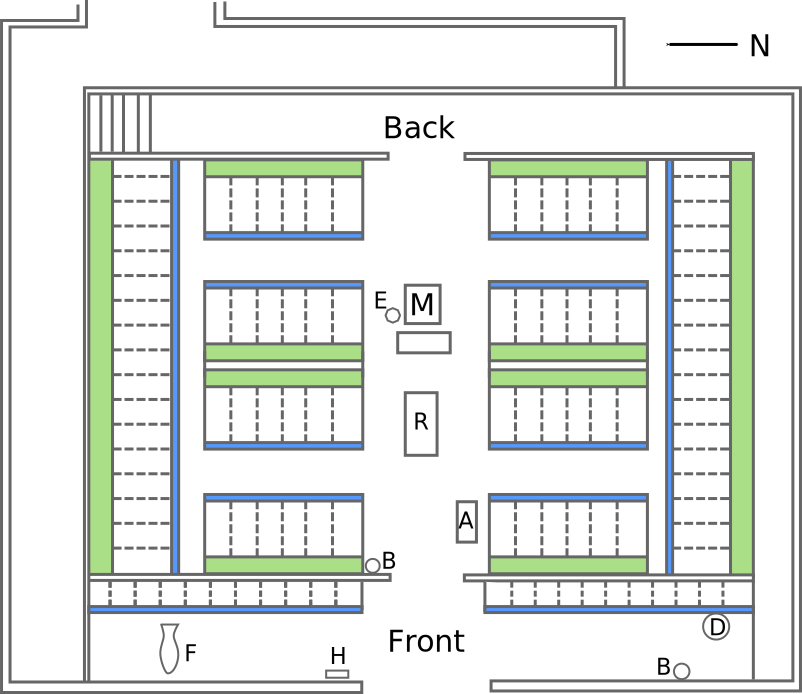
\includegraphics[width=\textwidth]{Soudou}
\end{center}

\clearpage

\begin{multicols}{2}

\section{Terms}

\paragraph{Abbot}

The J\=uji (住持), the head priest of a temple or monastery.

\paragraph{Attendant}

A jisha (侍者), a senior monk with particular responsibilities.

\paragraph{Cloud-shaped gong}

A cloud-shaped gong, or unpan (雲版), is a metal gong hit with a wooden mallet.

\paragraph{Dharma}

Dharma is a Sanskrit word often translated as ``teaching'', generally
Buddhist teaching of perfect truth. It can also refer to the cosmic
order or be used simply to refer to the way of doing something.

\paragraph{Gassh\=o (合掌)}

Hands together in front of face, fingertips even with the tip of your nose
and move with your head as you incline or bow. Arms and elbows out.

\paragraph{Hatsu-u (鉢盂)}

A set of nesting bowls used for meals, in modern times called
\=Ory\=oki (応量器). Modern S\=ot\=o Zen practitioners use up to 5 bowls, but
D\=ogen only mentions four bowls specifically.  The largest bowl,
called the zuhatsu (``head bowl'') and in modern English the ``Buddha
bowl'', has a round bottom and rests on a stand in the form of a small
flat-bottomed bowl.

\paragraph{Manjushri}

Manjushri is a Bodhisattva associated with wisdom. A statue of
Manjushri is given a central place in the Monks' Hall.

\paragraph{Okesa (御袈裟)}

A monk's over-robe, a formal garment sewed from strips, originally
made from discarded rags dyed uniformly.

\paragraph{Roll-downs}

Three roll-downs, san'e (三会), is a standard signal in the monastery.
It takes the form of 7 slow, evenly-spaced hits, a rapidly
accelerating series of hits, 5 slow hits, an accelerating series,
3 slow hits, and then one more accelerating series.

\paragraph{Shashu (叉手)}

A ritual hand position when standing or walking in formal contexts.
It can mean hands folded at chest height with forearms parallel to the
floor or hands flat against the chest with thumbs interlaced.

\paragraph{Supervisor}

The In\=o (維那), one of the six temple administrators that supervises
the monks' hall and the monks' conduct.

\paragraph{Zafu (坐蒲)}

A sitting cushion used for meals and sitting meditation. The term
is modern; D\=ogen actually uses the word ``futon''.

\vfill

\begin{center}

\includegraphics[height=1in]{Images/Green_Gulch_Farm_Dinner_Gong.jpg}

{\small A cloud-shaped gong\\
\scriptsize By Terrie Miller, CC-BY-SA-2.0, via Wikimedia Commons\par}

\vfill

\includegraphics[height=.75in]{Images/Zafu.jpg}

{\small A Zafu\\
\scriptsize By Dharamweb, CC-BY-SA-3.0, via Wikimedia Commons\par}

\end{center}

\columnbreak

\section{Texts}

\subsection{The Ten Names of Buddha}

The pure Dharmakaya Vairochana Buddha,\\
the complete Sambhogakaya Rushana Buddha,\\
the ten trillion forms Nirmanakaya Shakyamuni Buddha,\\
the future Maitreya Buddha,\\
all buddhas, ten directions, three times,\\
the Mahayana, \emph{Wondrous Dharma Lotus Flower Sutra},\\
the great wisdom Manjushri Bodhisattva,\\
the Mahayana Samantabhadra Bodhisattva,\\
the great compassion Avalokiteshvara Bodhisattva,\\
all venerable bodhisattva mahasattvas,\\
maha prajna paramita.

\subsection{The Meal Offering Verse, Breakfast}

The ten benefits of this morning meal\\
abundantly nourish practitioners\\
with unlimited rewards,\\
fulfilling eternal joy.

\subsection{The Meal Offering Verse, Lunch}

The three virtues and six tastes\\
we offer to buddha, sangha,\\
and all beings in the phenomenal world,\\
giving nourishment equally to everyone.

\subsection{The Five Contemplations}

First, regarding how great an effort [brought us this food]. we consider where it has come from.\\
Second, we reflect on whether our virtue and practice are worthy of receiving this offering.\\
Third, to protect the mind, abandoning our mistakes from greed, hate, and delusion is essential.\\
Fourth, truly this good medicine is for healing our fragile bodies.\\
Fifth, now we receive this food for the sake of accomplishing Buddha's way.

\subsection{Existing in the World\protect\footnote{Not written out in the text}}

Existing in the world like vast space, like a lotus flower not attached
to water, the Mind's purity goes beyond. We prostrate ourselves to the
unsurpassed World-Honored One.

\section{Meta}

I am Kih\=o, a wandering poet who presently abides in the Barony of
Carolingia. I may be contacted at \texttt{kihou@mit.edu}. In these
modern Middle Ages, I am not a monk or a serious Zen practitioner, so
do not treat my perspective as authoritative on such matters. I was
inspired to teach this class based on time I spent living briefly at a
Soto Zen monastery in France. I have a blog where I discuss period
Japan, \url{http://fireflies.xavid.us/}.

\section{Source}

\begin{description}
\cited
\end{description}

\end{multicols}

\end{document}
